\subsection{Análisis de los resultados del cálculo de las correlaciones}

Aplicando la ecuación  \ref{eq:corr_est}  para el estimador de la autocorrelación de la muestra discreta
se calcularon autocorrelaciones a distintas temperaturas y con distintos tamaños 
de matriz de espines. Se agruparon los resultados de manera de mostrar en un mismo
tamaño de matriz, diferentes temperaturas y en iguales temperaturas distintos tamaños de matriz.

\subsubsection{Correlación en función de la temperatura}

En la figura \ref{fig:corre_20x20}, se pueden ver los resultados del cálculo
de correlaciones para  temperaturas $T =9.0 $, $T = 1.0 $, $T =0.8 $ y $T = 2.3 $, en una matriz de tamaño 20x20.
En este caso con el descenso de la temperatura se observa un aumento del valor del parámetro
de correlación $\tau_{c}$.


\begin{figure}[H]
   \begin{center}
        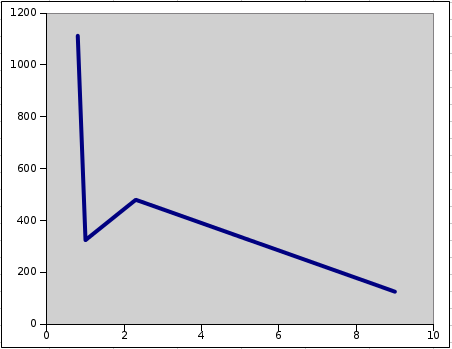
\includegraphics[scale=0.6]{corre_temperature.png} \\
        \caption{Parámetro de correlación  $\tau_{c}$ en función de la temperatura $T$}\label{fig:corre_tempe}
    \end{center}
\end{figure}


\subsubsection{Correlación en función del tamaño del problema}
En las figuras \ref{fig:corre_tamano_t2} y \ref{fig:corre_tamano_t9}, se pueden ver los resultados del cálculo
de correlaciones para los tamaños de matriz 20x20 y 100x100 para valores de $T = 2.3$  y $T = 9.0$. 
En los dos casos se observa un aumento del parámetro de correlación con el aumento del 
tamaño de la matriz de spines.

\section{Descripci\'on del sistema de c\'alculo}


Se desarrollo un c\'odigo de c\'alculo en Fortran y dos c\'odigos
en python uno  de pre y el otro de post-procesamiento. Tanto el código de preprocesamiento, 
como el código de postprocesamiento, comprenden varios módulos responsables de distintas
tareas.

El proyecto se encuentra bajo control de versión en un repositorio \textbf{git} de CNEA
y se obtiene con los permisos adecuados haciendo:

\begin{verbatim}
> git clone https://lpizarro@scmmanager.dcap.cnea.gov.ar/scm/git/SimRui
\end{verbatim}


Una vez cloneado el repositorio, para acceder al código, hacer:

\begin{verbatim}
  > cd FORTRAN/ising
\end{verbatim}



El c\'odigo fuente del programa \textbf{\textit{ising.f90}}, se encuentra en la carpeta
\textbf{src/}, su compilación se hace con el sistema \textbf{cmake} y depende
de un conjunto de módulos que se encuentra en la carpeta \textbf{libs}.

Para compilarlo hay que crear hacer:

\begin{verbatim}
  > mkdir build/
  > cd build/
  > cmake ..
\end{verbatim}

esas operaciones crean un directorio \textbf{bin/} donde se encuentran todos
los elementos necesarios para hacer las corridas del programa.
Para eso hay que parametrizar adecuadamente el sistema en \textbf{\textit{parametros.py}}.

Los comentarios del módulo explican el fin de cada una de las variables globales python.

\begin{verbatim}
# -*- coding: utf-8 -*-

###############################################################################       
#   PARAMETROS DE ENTRADA
###############################################################################
# Tamaño de la red de spines
N_red = 20
M_red = 20
# Cada cuántos puntos se quiere grabar el archivo temporal
# K_grab = 0 especifica que no se grabe ningún archivo temporal
N_grab = 0     
# Barrido de temperaturas
# Temperatura mínima
T_min = 0.5
# Temperatura máxima
T_max = 4.0
# Paso de temperatura
dT = 0.1
# Agrego el detalle cerca de la temperatura crítica
T_detail_min = 2.10
T_detail_max = 2.50
dT_detail = 0.02
# Número de pasos para la primer corrida (termalización)
N_term = '4000'
# Número de pasos para la segunda corrida (medición)
N_medi = '10000'
# Número de corridas para cada temperatura
Nrun = 8
#
# FIN PARAMETROS DE ENTRADA
###############################################################################

\end{verbatim}


y luego hacer, para correr la versión serie:

\begin{verbatim}
  > cd bin/
  > python corridas.py
\end{verbatim}

o si se quiere correr la versión paralelo:

\begin{verbatim}
  > cd bin/
  > python corridas_paralelos.py
\end{verbatim}

Luego de una corrida en una serie de temperaturas, queda una estructura de directorios
como la que se muestra en \ref{fig:arbol.dir}, con la información necesaria para postprocesar
los resultados y obtener los valores de las mediciones en función de la temperatura.

Una vez que se terminan los cálculos para todas las temperaturas,  en 
la carpeta \textbf{bin/}, se corre:

\begin{verbatim}
  > python grafico_tablas.py 
\end{verbatim}

para obtener los gráficos de las medidas fundamentales del sistema.

Si se quieren obtener los gráficos de las correlaciones a distintas temperaturas, 
se debe correr:

\begin{verbatim}
  > python correlaciones.py 
\end{verbatim}



\subsection{C\'odigo ising}

\subsubsection{Par\'ametros de entrada}

El programa ising lee la configuraci\'on de una corrida del 
archivo parametros.dat que tiene que estar en la carpeta donde se
corre ising.

El archivo \textbf{parametros.dat} tiene la forma: 

\begin{verbatim}
     N M T J MCS PE. 
\end{verbatim}

Donde NxM 
son las dimensiones de la matriz, T la temperatura de la corrida,
J el par\'ametro de c\'alculo de energ\'ia de Ising, MCS son los pasos Monte Carlo y PE
es una cantidad que especifica cada cuantos pasos Monte Carlo se graba la energ\'ia.

\begin{verbatim}
   20 20 2.22 1 500 100
\end{verbatim}


\paragraph{Preprocesamiento en python}
En la carpeta \textbf{src/} el archivo parametros.py contiene la parametrizaci\'on 
de los scripts
en python que permiten correr el sistema en serie (ver \ref{serie}), 
o en paralelo (ver \ref{paralelo}).
El preprocesamiento en python, permite definir una zona de c\'alculo de paso
de temperatura fino. Es decir se puede parametrizar un paso de temperatura de
0,1 para todo el rango de temperatura y dentro de ese rango definir una zona
donde el paso de temperatura puede ser menor, ej. $\Delta T$ = 0.01. Para lograr una mejor resoluci\'on
en esa zona.

En particular en este c\'alculo se uso para explorar con m\'as detalle la zona
cr\'itica.

El preprocesamiento en python, crea el archivo parametros.dat, 
 corre el programa de ising a distintas temperaturas
  Crea una carpeta para cada temperatura. En cada una de esas carpetas, a su
  vez, crea Nruns carpetas para hacer estadística y obtener los valores con
  sus respectivos errores.
 
  En cada temperatura, se utiliza el valor final de la temperatura anterior.
  Arbitrariamente, se toma el valor final de RUN00 como el valor inicial de
  todas las corridas a la siguiente temperatura (menor)
 

\subsubsection{Salida del programa}

Los resultados los guarda en el archivo tablas\_temperatura.dat.

Cada fila de tablas\_temperatura.dat representa los resultados a una dada
temperatura con sus respectivos errores. Las columnas son:

\begin{verbatim}
  T <E> std(E) <M> std(M) <c> std(c) <suc> std(suc) <acept> std(acept)
\end{verbatim}

Donde:



\begin{itemize}
  \item $T$: temperatura de la corrida 
    \item $<E>$: Energ\'ia media calculada
    \item  $std(E)$: desviaci\'on standard de la energ\'ia calculada

    \item $<M>$: Magnetizaci\'on media calculada
    \item  $std(M)$: desviaci\'on standard de la Magnetizaci\'on calculada


    \item $<c>$: Capacidad calor\'ifica media calculada
    \item  $std(c)$: desviaci\'on standard de la Capacidad calor\'ifica calculada

    \item $<suc>$: Susceptibilidad magn\'etica media calculada
    \item  $std(suc)$: desviaci\'on standard de la Susceptibilidad magn\'etica calculada


    \item $<acept>$: Aceptaci\'on media calculada
    \item  $std(acept)$: desviaci\'on standard de la Aceptaci\'on calculada
\end{itemize}



  Los errores se calculan como $std(RUN)/sqrt(NRUN)$


\subsubsection{Librer\'ias utilizadas}

La carpeta \textbf{libs/} contiene las librer\'ias usadas por el sistema

\paragraph{\underline{\textit{estadistica.f90}}}

Un conjunto de subrutinas para c\'alculo estad\'istico. 

\paragraph{\underline{\textit{globales.f90}}}
Un m\'odulo que contiene las variables globales del programa.
	
\paragraph{\underline{\textit{io\_parametros.f90}}}  
Un m\'odulo para el manejo de la entrada y las salidas de los
datos del programa.


\paragraph{\underline{\textit{isingmods.f90}}} 
En este m\'odulo  se encuentran las principales rutinas de c\'alculo del
sistema.


\paragraph{\underline{\textit{strings.f90}}}
Un m\'odulo que contiene subrutinas de manejo de cadena de caracteres.


\paragraph{\underline{\textit{usozig.f90}}} 
En este m\'odulo se ecuentran las subrutinas que usan ziggurat y que
son usadas en el programa principal, ising.
					
					
\paragraph{\underline{\textit{ziggurat.f90}}}

Para la generaci\'on de n\'umeros aleatorios se utilizaron
las capacidades provistas por la librer\'ia ziggurat. 


\subsection{Corridas en serie}\label{serie}
El módulo python \textbf{\textit{corridas.py}}, es el que tiene la capacidad de correr
el código de cálculo en una máquina con un único núcleo. Parametrizando adecuadamente
\textbf{\textit{parametros.py}} se logran tiempos de corrida razonables en una máquina
con un único procesador. El parámetro que permite acelerar la velocidad de porcesamiento, 
es el que indica cada cuantos pasos Monte Carlo, se quieren grabar las energías.

\subsection{Corridas en paralelo}\label{paralelo}

El módulo python \textbf{\textit{corridas\_paralelos.py}}, es el que tiene la capacidad de correr
en una máquina con varios núcleos.

El código se paraleliza usando el paquete \href{http://mpi4py.scipy.org/} {\textbf{mpi4py}} ,  desarrollado por Lisandro Dalcin.
De esa manera lo que se hizo, es paralelizar desde python y no desde Fortran.

El criterio utilizado para paralelizar es hacer en simultaneo  las corridas a una dada temteratura. 
Una vez que terminan los cálculos a una dada temperatura, se hacen los cálculos en la próxima
temperatura con el estado final de la temperatura anterior.

Este diseño permitió hacer cálculos en sistemas de mayor tamaño, lograndose llegar a dimensiones
de 100x100. De esa manera se obtuvieron las curvas que muestran el comportamiento del sistema en
tamaños mayores a 20x20.
